\chapter{图像生成模型}
\label{cha:sysu-thesis-contents-format-requirement}

\section{对抗生成模型}
生成式对抗网络(generative adversarial networks,GAN)是一种深度学习模型,由Ian Goodfellow等人于2014年提出。
在GAN模型之前,生成模型主要基于概率图模型、隐变量模型等方法,如概率生成模型和自动
编码器。这些方法在生成样本时面临着训练困难和生成样本质量低下的问题。
生成对抗网络引入了对抗博弈的思想,通过对抗训练的方式,同时训练生成器和判别器,实现生成高质量样本的能力。

作为基于博弈的生成模型,GAN主要由生成器与判别器两部分组成。核心思想是通过让生成器生成逼真的样本,以欺骗判别器来提高生成器的能力。
生成器接受一个随机向量作为输入,并通过一系列的转换将其映射到数据空间中。判别器则负责对生成器
生成的样本和真实样本进行区分。通过不断迭代训练,生成器能够逐渐学习到生成高
度逼真的样本,这些样本在视觉上几乎无法与真实数据区分开来。

\begin{figure}[!htbp]
    \centering
    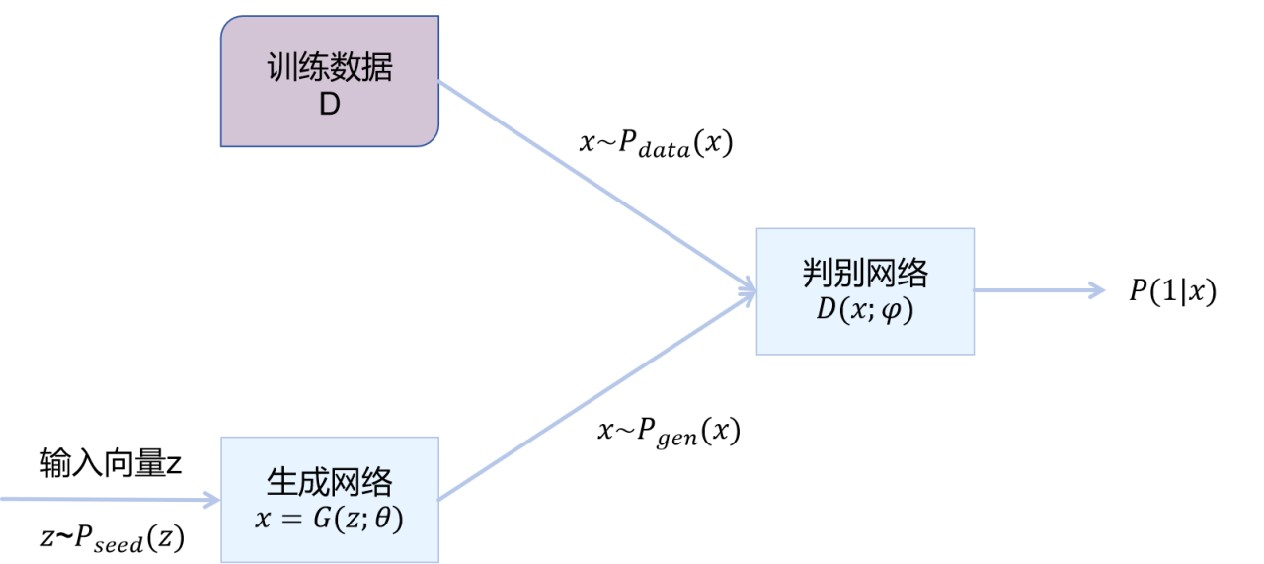
\includegraphics[width=10cm]{image/chap02/GAN.jpg}
    \label{fig:GAN}
\end{figure}

其中$x$表示需要学习的真实数据,服从分布$P_{data}(x)$;
$z$表示随机输入的噪声,服从分布$P_{seed}(z)$;
$G(z;\theta)和D(x;\phi)$分别表示生成网络和判别网络。

判别网络和生成网络形成博弈关系,得到GAN的学习目标函数:
$$\underset{\theta}{min}\underset{\phi}{max}\left\{E_{x\sim P_{data}(x)}[logD(x;\phi)]+E_{z\sim P_{seed}(z)}[log(1-D(G(z;\theta);\phi)]\right\}$$

\subsection{算法流程图}
\label{sec:algorithm}
\begin{algorithm}[h]
    \KwIn{训练数据$D$}
    
    \caption{生成对抗网络算法}
    \label{algo:sgd}
\end{algorithm}

\section{扩散模型}
扩散模型受热力学扩散启发,模拟数据从有序到无序(添加噪声)再恢复有序(去除噪声)的过程。
\cite{ho2020denoising}
具体分为两个阶段:

1)前向过程(扩散过程):逐步向数据中添加高斯噪声,最终使数据变为纯噪声。

2)反向过程(去噪过程):通过神经网络学习逐步去除噪声,从噪声中重建原始数据。

\subsection{字体和字号的说明}

标题一般用黑体,内容一般用宋体,数字和英文字母一般用Times New Roman,具体如\autoref{tab:font-spec}。

\begin{table}[]
    \caption{字体使用规范}
    \begin{tabular}{|c|c|}
        \hline
        论文题目               & 黑体二号居中                                  \\ \hline
        中文摘要标题           & 黑体三号居中                                  \\ \hline
        中文摘要内容           & 宋体小四号                                    \\ \hline
        中文关键词             & 宋体小四号(标题``关键词''加粗)              \\ \hline
        英文摘要标题           & Times New Roman加粗三号全部大写               \\ \hline
        英文摘要内容           & Times New Roman小四号                         \\ \hline
        英文关键词             & Times New Roman小四号(标题``Keywords''加粗) \\ \hline
        目录标题               & 黑体三号居中                                  \\ \hline
        目录内容               & 宋体小四号                                    \\ \hline
        正文各章标题           & 黑体三号居中                                  \\ \hline
        正文各节一级标题       & 黑体四号左对齐                                \\ \hline
        正文各节二级及以下标题 & 宋体小四号加粗左对齐空两格                    \\ \hline
        正文内容               & 宋体小四号                                    \\ \hline
        参考文献标题           & 黑体三号居中                                  \\ \hline
        参考文献内容           & 宋体五号                                      \\ \hline
        致谢、附录标题         & 黑体三号居中                                  \\ \hline
        致谢、附录内容         & 宋体小四号                                    \\ \hline
        页眉与页脚             & 宋体五号居中                                  \\ \hline
        图题、表题             & 宋体五号                                      \\ \hline
        脚注、尾注             & 宋体小五号                                    \\ \hline
    \end{tabular}
    \label{tab:font-spec}
\end{table}


字体样例可见如下(以居中形式展现): \\

\begin{center}
    {\heiti\zihao{2}黑体二号居中} \\

    {\heiti\zihao{3}黑体三号居中} \\

    {\heiti\zihao{4}黑体四号居中} \\

    {\songti\zihao{4}宋体四号居中} \\

    {\songti\zihao{-4}宋体小四号居中} \\

    {\songti\zihao{5}宋体五号居中} \\

    {\songti\zihao{-5}宋体小五号居中} \\

    {\zihao{3} Times New Roman : Three} 三号居中 \\

    {\zihao{-4} Times New Roman : Small Four} 小四号居中 \\

\end{center}


\subsection{页面设置}

纸张大小:A4。

页边距:上边距25 mm,下边距20 mm,左右边距均为30 mm。

行距:1.5倍行距,章和节标题段前段后各空0.5行。

\subsection{页码}

页面底端居中,从摘要开始至绪论之前以大写罗马数字(
\uppercase\expandafter{\romannumeral1} ,
\uppercase\expandafter{\romannumeral2} ,
\uppercase\expandafter{\romannumeral3} ,
…)单独编连续码,绪论开始至论文结尾,以阿拉伯数字(1,2,3…)编连续码。

\subsection{关键词}


摘要正文下方另起一行顶格打印``关键词''款项,后加冒号,多个关键词以逗号分隔。

\subsection{目录}

目录应另起一页,包括论文中的各级标题,按照``一……''、``(一)……''或``1……''、``1.1……''格式编写。

\subsection{各级标题}

正文各部分的标题应简明扼要,不使用标点符号。论文内文各大部分的标题用``一、二……(或1、2……)'',次级标题为``(一)、(二)……(或1.1、2.1……)'',三级标题用``1、2……(或1.1.1、2.1.1……)'',四级标题用``(1)、(2)……(或1.1.1.1、2.1.1.1……)'',不再使用五级以下标题。两类标题不要混编。


这是一个例子:

\begin{equation}
    \label{eq:example-formulas}
    ax^2 +bx+c = 0
\end{equation}


如\autoref{eq:example-formulas}所示,为了求解该一元二次方程,我们可以推导得到该方程的求根公式。因此,由\autoref{eq:example-formulas2}即可求解该方程的两个根。

\begin{equation}
    \label{eq:example-formulas2}
    \begin{split}
        x_1 = & \frac{-b+\sqrt{b^2-4ac}}{2a} \\
        & \\
        x_2 = & \frac{-b-\sqrt{b^2-4ac}}{2a}
    \end{split}
\end{equation}

\subsection{表格}

\begin{enumerate}
    \item 表格必须与论文叙述有直接联系,不得出现与论文叙述脱节的表格。表格中的内容在技术上不得与正文矛盾。
    \item 每个表格都应有自己的标题和序号。标题应写在表格上方正中,不加标点,序号写在标题左方。
    \item 全文的表格可以统一编序,也可以逐章单独编序。采用哪一种方式应和插图、公式的编序方式统一。表序必须连续,不得跳缺。
    \item 表格允许下页接写,接写时标题省略,表头应重复书写,并在右上方写``续表××''。多项大表可以分割成块,多页书写,接口处必须注明``接下页''、``接上页''、``接第×页''字样。
    \item 表格应放在离正文首次出现处最近的地方,不应超前和过分拖后。
\end{enumerate}


例子可见\autoref{tab:table-example}。

\begin{table}[!htbp]
    \centering
    \caption{表格例子}
    \label{tab:table-example}
    \begin{tabular}{|l|l|}
        \hline
        \multicolumn{1}{|c|}{这是表格第一行第一列} & 这是表格第一行第二列 \\ \hline
        这是表格第二行第一列                       & 这是表格第二行第二列 \\ \hline
    \end{tabular}
\end{table}


\begin{figure}[!htbp]
    \centering
    \includegraphics[width=3cm]{example-image-a}
    \caption{图片例子}
    \label{fig:example-figure}
\end{figure}

\subsection{注释}

毕业论文(设计)中有个别名词或情况需要解释时,可加注说明。注释采用脚注或尾注,应根据注释的先后顺序编排序号。注释序号以``①、②''等数字形式标示在正文中被注释词条的右上角,脚注或尾注内容中的序号应与被注释词条序号保持一致。

脚注例子可见这里\footnote{这是一个脚注}。


\subsection{附录}

论文附录依次用大写字母``附录A、附录B、附录C……''表示,附录内的分级序号可采用``附A1、附A1.1、附A1.1.1''等表示,图、表、公式均依此类推为``图A1、表A1、式A1''等。

% TODO:增加引用例子。